\documentclass{article}
\usepackage{import}
\subimport{../}{preamble}
\begin{document}

\section{Plasmon Coupling}
% ideas of scale invariance

% Basic introduction to charge interaction and gap modes
Both the resonant field enhancement and the confinement of a surface plasmon can be improved by bringing a second surface plasmon into close proximity. Similar to coupled harmonic oscillators and dipoles, plasmons couple together via Coulomb forces once brought together, forming normal modes of oscillation across interacting charge distributions. The charge distribution of the resulting normal modes depends highly on the particle separation and is strongly confined to the dielectric space between metallic surfaces where charges strongly interact. These normal modes are therefore more generally known as \emph{gap plasmons} and lead to tuneable \glspl{spr} \cite{huang2010, millyard2012} and significant increases in field enhancement, enabling single molecule spectroscopy \cite{mertens2013, taylor2014}.

Coupled plasmons are a feature of many metallic nano-systems with closely spaced metal-dielectric interfaces, including \gls{mim} and \gls{imi} waveguides \cite{maier2007plasmonics, lindquist2013} and systems containing multiple \glspl{mnp} \cite{maier2002, atay2004, muskens2007, huang2010, millyard2012, taylor2011, herrmann2013} or \glspl{npom} \cite{okamoto2003, daniels2005, kinnan2007, mubeen2012, mertens2013, denijs2014}. For the purposes of this work, discussion is restricted to the ideal case of coupled \glspl{lsp} between two closely spaced \glspl{mnp}, closely representing the experimental system, though the description of coupling is valid for many other cases involving \glspl{sp}.

\subsection{Localised Surface Plasmon Coupling in Nano-Gap Cavities}

In the simplest case, only multipolar plasmons, excited in two spherical \glspl{mnp} being driven by external \gls{em} fields, are considered. This is the prototypical plasmonic dimer system used to understand plasmon coupling. Similar systems, including chains and arrays of \glspl{mnp} \cite{maier2002, muskens2007, millyard2012} and \glspl{mnp} on mirrors \cite{okamoto2003, daniels2005, kinnan2007, mubeen2012, mertens2013, denijs2014}, have been used to study plasmon coupling. In each of these systems, the physics can be reduced to interactions between neighbouring charge distributions. This is why the simple dimer system is important to fully understand even more complex geometries.

The behaviour of a plasmonic dimer stems from the Coulomb interaction between free electrons in adjacent metallic nanostructures. As \glspl{mnp} move closer together the force between charges grows, increasingly polarising the local gap region to which the charge becomes confined. The introduction of separation-dependent forces to the plasmon oscillator shifts the resonance frequency of the individual plasmon mode from $\omega_0$ by $\Delta\omega$ depending on the strength of coupling. Since coupling is between multipolar fields, the relative orientation between excited \glspl{lsp} and the external driving field is important to determine the sign and strength of coupling.
%%%
In general, two coupled charge distributions can exist: an in-phase mode and an anti-phase mode. Compelling evidence for this has been seen many times since studying chains of AuNPs in 2002 \cite{maier2002}.
%%%
Coupling is strongest when adjacent plasmon poles are oppositely charged. This is generally the case for \glspl{lsp} in a \gls{mnp} dimer being driven in phase with the incident field.

% Field enhancement increase
The primary effect of gap plasmon excitation is the localisation of the electric field to the dielectric gap medium. As stated previously, a plasmon intrinsically enhances the near-field around a \gls{mnp}, caused by optically-driven charge accumulation at the metal-dielectric interface. For the case of two interacting plasmonic particles, the Coulomb forces between plasmons pulls charge more towards the gap region. As a result, a greater amount of charge accumulates on the metal surfaces around the gap and the field in the gap cavity becomes more localised and further enhanced.
%\footnote{This is much like with charged plates in a capacitor and how the field increases with dielectric gap material, spacing and charge accumulation.}
For a strongly confined gap mode there is very little field in the metal with almost all field confined within a small lateral mode within the gap \cite{romero2006}. This is known as a plasmonic ``hot spot". Through this mechanism alone the field enhancement $\left|E/E_0\right|$ can be increased by more than an order of magnitude \cite{hao2004, talley2005}. Hence, in recent years, the interests of the plasmonics community has shifted from individual plasmonic nanostructures to coupled systems in order to {\color{red}maximise nano-optical performance}.

\begin{figure}[bt]
\centering
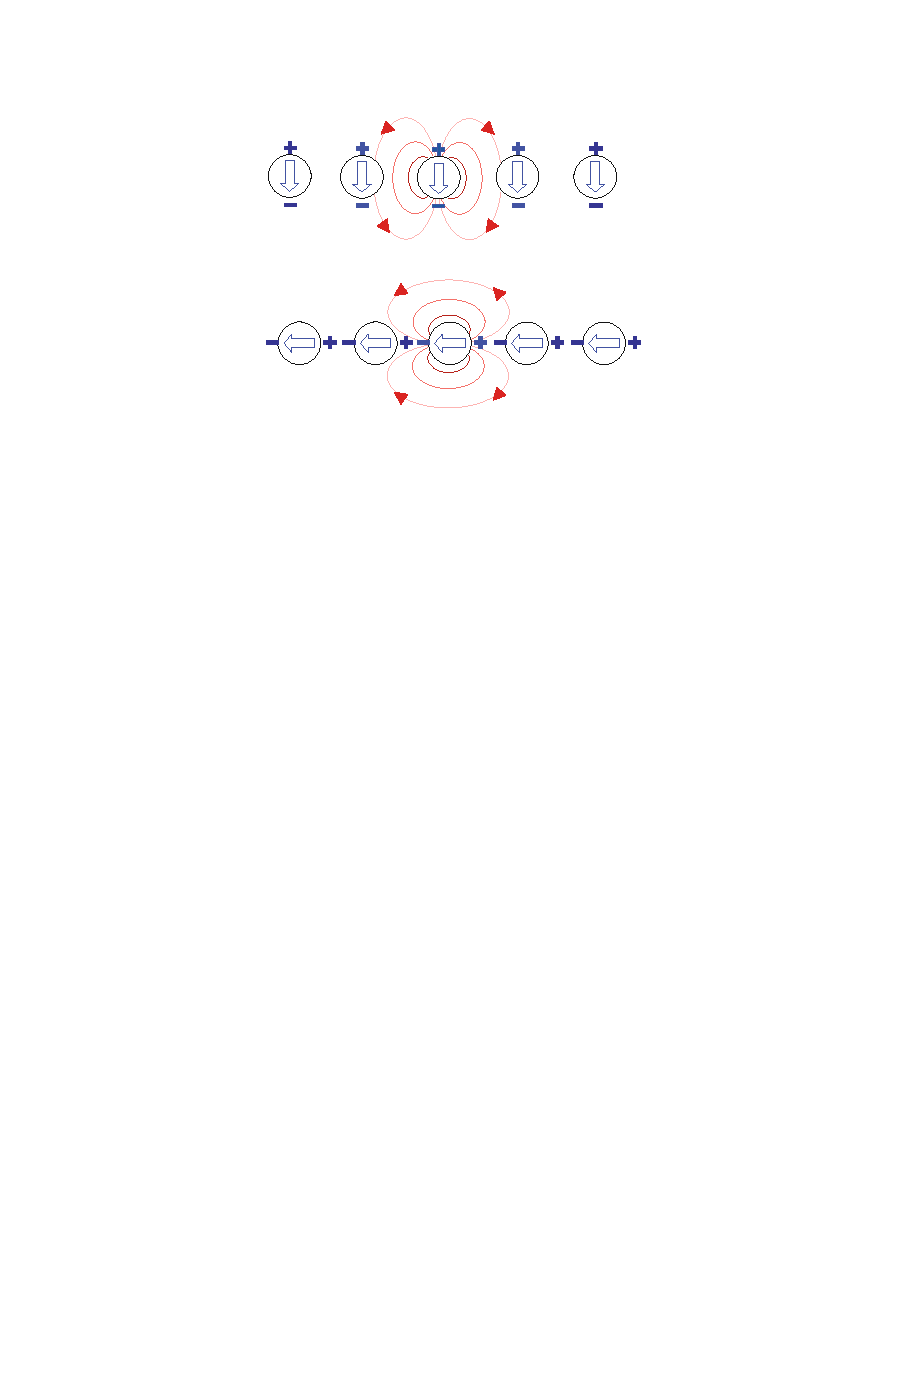
\includegraphics[width=0.45\textwidth]{figures/literature/maier_plasmonics_coupling_diagram}
\quad
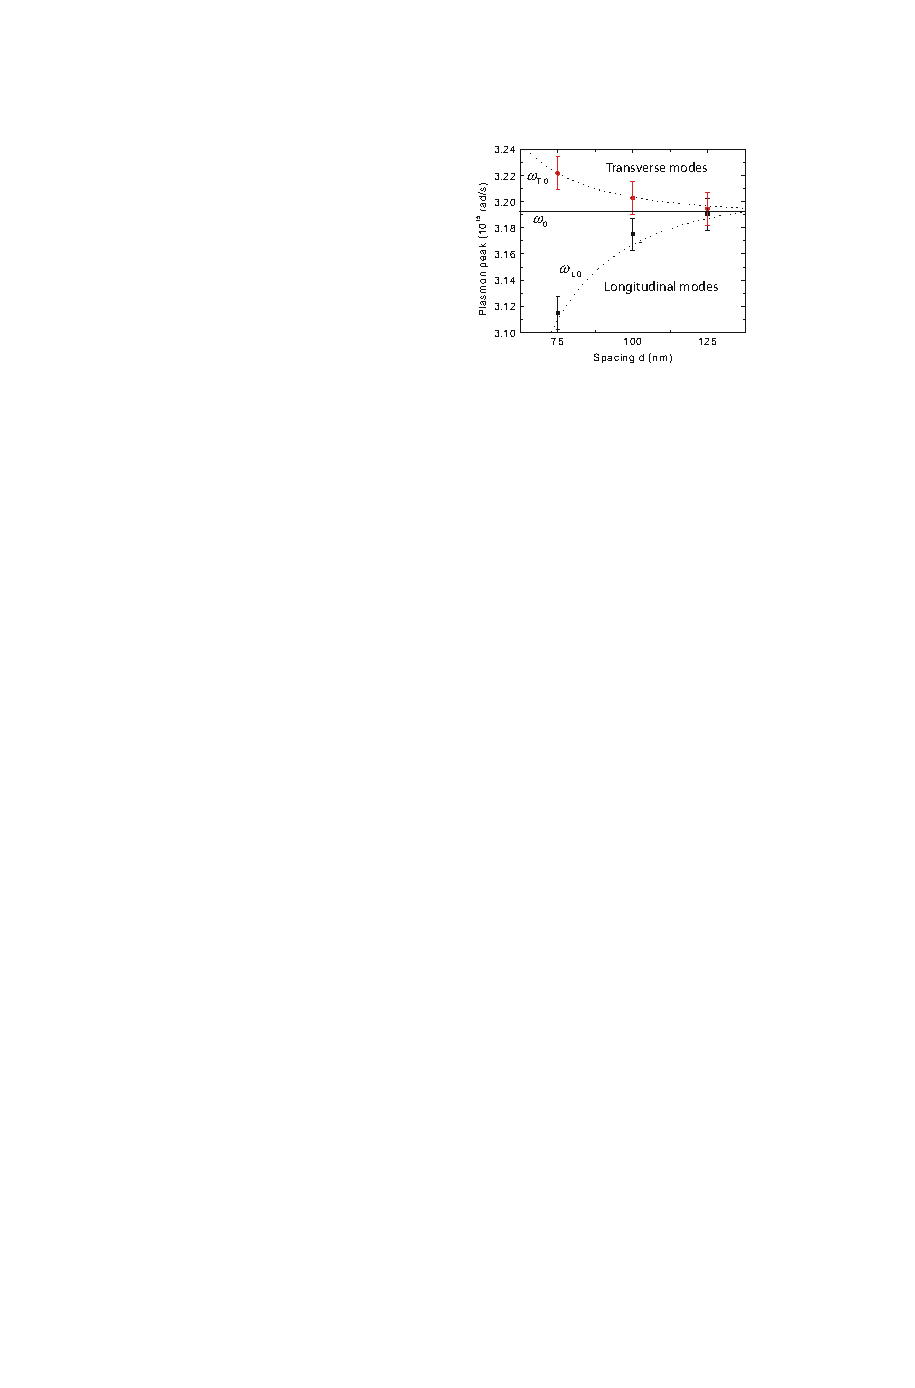
\includegraphics[width=0.45\textwidth]{figures/literature/maier_plasmonics_coupling}
\caption[Experimental and theoretical plasmon coupling]{\textbf{Experimental and theoretical plasmon coupling.} Dipolar plasmons in chains of spherical AuNPs couple depending on field orientation \cite{maier2007plasmonics} (left). Experimentally measured plasmon resonance energies in coupled AuNP chains show the gap-dependent tuning due to coupling \cite{maier2002} (right). The dotted line corresponds to a $r^{-3}$ point dipole model.}
\label{fig:maier_plasmon_coupling}
\end{figure}

% Experimental evidence
%Systems of AuNPs were experimentally studied from 2002 \cite{maier2002}, in which the individual resonances of AuNP chains with different spacings were shown to couple and form two new modes, gradually separating in energy with increased coupling strength (\figurename~\ref{fig:maier_plasmon_coupling}). Modes are identified as in-phase coupled modes between particles in orthogonal polarisations, for which resonances along the chain redshift while resonances perpendicular to the chain blueshift with decreased particle spacing. % Similar behaviour is observed for...

%\begin{wrapfigure}{O}{0.35\textwidth}
%\vspace{-10pt}
\begin{figure}[bt]
\fontsize{10pt}{1em}\selectfont
\def\svgwidth{0.7\textwidth}
\subimport{./figures/}{dipole_interactions.pdf_tex}
\caption[Diagram of dipole interactions]{\textbf{Diagram of dipole interactions.} Dipoles have length $D$. The distance between dipoles is $r$ with an edge-to-edge separation $d$. Configurations 1 and 3 are comparable with plasmon coupling as a result of sub-wavelength structures being driven by a single external light field. {\color{red}Configurations 2 and 4 are generally unphysical without significantly increasing the system size to create the necessary phase retardation for excitation. Even then the modes remain non-radiative due to zero net dipole moment.}}
\label{fig:dipole_interactions}
%\vspace{-5pt}
%\end{wrapfigure}
\end{figure}

% Beginning of theoretical descriptions
Over the last decade theory has quickly progressed to better describe and understand the optical response of coupled plasmons. Depending on the size and geometry of the dimer system, multiple theoretical descriptions and approximations are valid. Each of these models, along with the cases in which they remain valid, are henceforth described up until the most recent theories required to understand the effects induced by the addition of quantum tunnelling.

\subsubsection{Classical Description of Plasmon Coupling}

In its simplest case, interactions between dipolar plasmons in small \glspl{mnp} appear similar to dipole-dipole interactions \cite{kreibig1995optical, maier2002, gluodenis2002, rechberger2003, atay2004}. These exhibit the same behavioural dependence on separation and relative orientation with respect to the incident field. Hence, for small \glspl{mnp} in which only dipolar plasmons are present, plasmons can simply be considered to be dipoles with shifted resonances resulting from proximity to the other dipole. Examples of some commonly considered dipole-dipole interaction geometries are shown in \figurename~\ref{fig:dipole_interactions}. In each situation the electric field incident on a dipole $\vec{p_1}$ is perturbed by the presence of a second dipole $\vec{p_2}$ a distance $r$ away, resulting in an effective field given by \cite{},
\begin{subequations}
\begin{align}
	\vec{E}_{||}^1 &= \vec{E}_{0,||} + \frac{\vec{p}_2}{2\pi\epsfs\epsdi r^3}, \label{eq:par_coupling} \\
	\vec{E_{perp}^1} &= \vec{E_{0,perp}} - \frac{\vec{p_2}}{4\pi\epsfs\epsdi r^3}. \label{eq:perp_coupling}
\end{align}
\end{subequations}
The sign of the second term in each equation determines the effect of coupling whilst its strength falls as $r^{-3}$ due to $V \propto p_1p_2r^{-3}$ \cite{halas2011}. Attractive coupling, as in \eqref{eq:par_coupling}, increases the local field at the dipole whereas repulsive coupling, as in \eqref{eq:perp_coupling}, has the opposite effect.
For two parallel, oscillating dipoles aligned end-to-end and driven in phase, coupling is attractive, leading to a decrease (redshift) of the resonant frequency. Conversely, the interaction between two parallel dipoles aligned side-by-side is repulsive, causing an increase (blueshift) of the resonant frequency. However, a symmetric anti-phase configurations leads to no net dipole moment and local field cancellation. Optical observation of such modes is then only possible for non-symmetric dipole-dipole systems. Experimental verification of this behaviour for each dipole configuration was therefore carried out using \gls{eels} on AuNP chains, showing the validity of the simple dipole approximation \cite{maier2002}.
%Alternatively, for dimers outside of the quasistatic regime, phase retardation of the driving field across the dimer is capable of breaking the coupling symmetry, allowing these modes to be excited.

The dipole-dipole model is improved to better describe a \gls{mnp} dimer by taking into account the finite particle size. Since the internal restoring force within particles, scaling as $D^3$, contributes to the potential, the interaction energy goes as $(r/D)^{-3}$ as opposed to $r^{-3}$ \cite{jain2007}. Furthermore, this quantity is redefined to better represent a coupled \gls{mnp} dimer using the gap size, \gls{d}, as $(d/D) = (r/D)-1$ rather than the centre of mass separation. The resonant wavelength shift due to attractive coupling can then be described using a ``plasmon ruler" equation \cite{jain2007, ben2011},
\begin{equation}
	\frac{\Delta\lambda}{\lambda_0} = a\exp{\left[-\frac{(d/D)}{\tau}\right]},
	\label{eq:plasmon_ruler}
\end{equation}
where $a$ is the coupling strength and $\tau$ is a decay constant. The exponential decay well approximates the more complex $(d/D)^{-3}$ behaviour, which is expressed in terms of shape and size parameters, $\Lambda$ and $\gamma$, as,
\begin{equation}
	\frac{\Delta\lambda}{\lambda_0} = \frac{1}{12\Lambda(d/D+1)^3 - (1-\gamma)}.
\end{equation}
In essence, this model and the dipole-dipole model both describe a similar phenomenon - that dimers comprised of larger particles interact more strongly for the same separation. The larger surfaces lead to a stronger capacitive interaction, or in the dipole model the amount of charge incorporated into $\vec{p}$ is increased. In recent years this relation still shows good agreement with experimental data but the approach remains limited to describing only dipolar modes in simple geometries \cite{muskens2007}. % add citation?

% Plasmon hybridisation theory
\begin{figure}[bt]
\centering
\fontsize{10pt}{1em}\selectfont
\def\svgwidth{0.98\textwidth}
\subimport{./figures/}{plasmon_dimer_hybridisation.pdf_tex}
\caption[Diagram of plasmon hybridisation between coupled plasmons in a nanoparticle dimer]{\textbf{Diagram of plasmon hybridisation between coupled plasmons in a nanoparticle dimer.} Plasmons are coupled along the dimer axis. Coupling leads to bonding and anti-bonding modes for each set of interacting $l$ modes (left). Interaction with higher order $l$ modes lowers the overall energy of lower order coupled modes (green lines). Only the bonding ($\omega_{\uparrow\uparrow}$) mode in the symmetric (homo-)dimer has a net dipole moment and is therefore observable. Cancellation of the net dipole moment means the anti-bonding ($\omega_{\uparrow\downarrow}$) mode remains optically dark. On the contrary, asymmetry in a (hetero-)dimer means both modes stay bright (right). In this case, the lower and higher energy individual modes shift to form the bonding and anti-bonding hybridised modes, respectively. This diagram is adapted from \cite{nordlander2004}.}
\label{fig:plasmon_hybridisation}
\end{figure}

A slightly more complex model, known as plasmon hybridisation, was developed between 2003 and 2004 to more generally explain the formation and behaviour of coupled modes \cite{prodan2003, prodan2004, nordlander2004}. In this model plasmon resonances are mechanically modelled as resonant oscillations of an incompressible fluid confined within an equilibrium geometry \cite{prodan2004}. The plasmon resonances of more complex particle geometries are then solved by decomposing it into coupled resonances of two simpler particle geometries \cite{prodan2003, prodan2004}. This is done in analogy with the ideas underpinning molecular orbital hybridisation and the hybridisation of quantum energy states. Using this logic, the theory equally describes the plasmon resonances of two coupled simple particle geometries \cite{nordlander2004} or a particle coupled with its image charge in a surface \cite{nordlander2004a}. Under these circumstances, the multipolar modes of each of the individual dimer particles energetically split into two hybridised modes representing the bonding (in-phase) and anti-bonding (anti-phase) configurations. This behaviour is shown in \figurename~\ref{fig:plasmon_hybridisation}.

% bonding vs anti-bonding
Unlike the dipole-dipole model, plasmon hybridisation is capable of predicting higher order multipolar modes in a coupled dimer system as well as dealing with more complex geometries. It is therefore valid for describing larger dimer geometries and smaller gap sizes. As with dipole-dipole interactions, the bonding and anti-bonding hybridised modes redshift and blueshift from their initial mode positions upon decreasing the separation, respectively. However, the addition of higher order modes to the classical description of plasmon coupling, and their interaction with adjacent modes of similar energies, modifies the rates of each mode's shift, as shown by the green lines in \figurename~\ref{fig:plasmon_hybridisation} \cite{nordlander2004}. These interactions leads to a further redshift of each affected mode, though only in the case of small gaps or larger particles when higher order modes are excited.

In each classical approach it is the resulting dipole moment of each coupled mode that dictates its radiative properties. The in-phase, bonding mode exhibits a large dipole moment and strongly interacts with light whereas the anti-phase, anti-bonding mode has no net dipole moment in a symmetric, quasistatic system and thus remains dark. This remains the case until the anti-bonding dimer mode acquires a finite net dipole moment, either through particle asymmetry (difference material, size or shape) or phase retardation (large particles, non-quasistatic)%
\footnote{Phase retardation of the driving field across the dimer breaks the coupling symmetry, allowing anti-phase modes to be excited.}%
, at which point it becomes more radiative and hence experimentally observable using optical methods. Alternatively, local excitation of specific charge distributions using \gls{eels} allows for measurement of dark modes \cite{chu2008, koh2009}.

Whilst each of the previously described analytical models has found some success in describing experimentally observed plasmon coupling in simple systems, their approaches are limited in scope. Neither model directly calculates electrodynamics and solves the actual electromagnetic problem. Instead, they use analogies to similar electromechanical systems to provide a useful insight into the mechanism of plasmon coupling. This is primarily due to the difficulty in analytically solving electrodynamics. Regardless, experimental plasmonic geometries are continually decreasing in size and solving the electrodynamics is necessary to accurately describe each system. As a result, computationally demanding, numerical techniques are applied to solve electrodynamics at each boundary within a system.

%Classically, for nm-size gaps, a whole range of higher order modes are expected to exist in the gap \cite{romero2006}. The lateral confinement of these modes across the gap is estimated using as $\sqrt{Rd}$. 
%As with dipole coupling, an opposite effect occurs when the driving field is orientation perpendicular to the dimer axis. In this instance the excited plasmon poles repel each other more with decreasing separation and the bonding mode therefore blueshifts \cite{gunnarsson2005, yang2010}.

\subsection{The Dynamical Optical Response of Plasmonic Dimers: Transitioning from Capacitive to Conductive Plasmonic Coupling}
% \cite{kadkhodazadeh2013} should go in last chapter, \cite{elkhoury2014} maybe to include

Using modern numerical simulation techniques, such as the \gls{bem} and \gls{fdtd} approaches, the full separation-dependent optical response of a plasmonic dimer has been calculated as particles transition from non-interacting to coupled through into geometrical contact \cite{romero2006}. In these calculations, the lowest order plasmons hybridise, redshift and more intensely scatter as the separation decreases, with higher order modes eventually emerging. Classically, this leads to a large number of modes being present in nanometric-size gaps. The lateral confinement of the field between particles of radius $R$ separated by a gap of width $d$ is estimated using $\sqrt{Rd}$ \cite{romero2006}. As higher order modes become more intense, scattering from lower order modes decreases. Despite this, their field enhancement continues to rise. These plasmons become so confined that they no longer couple with the far-field. This behaviour continues until the particles are nearly touching into geometrical contact. % check this with Jeremy's counterargument!

\begin{figure}[bt]
\centering
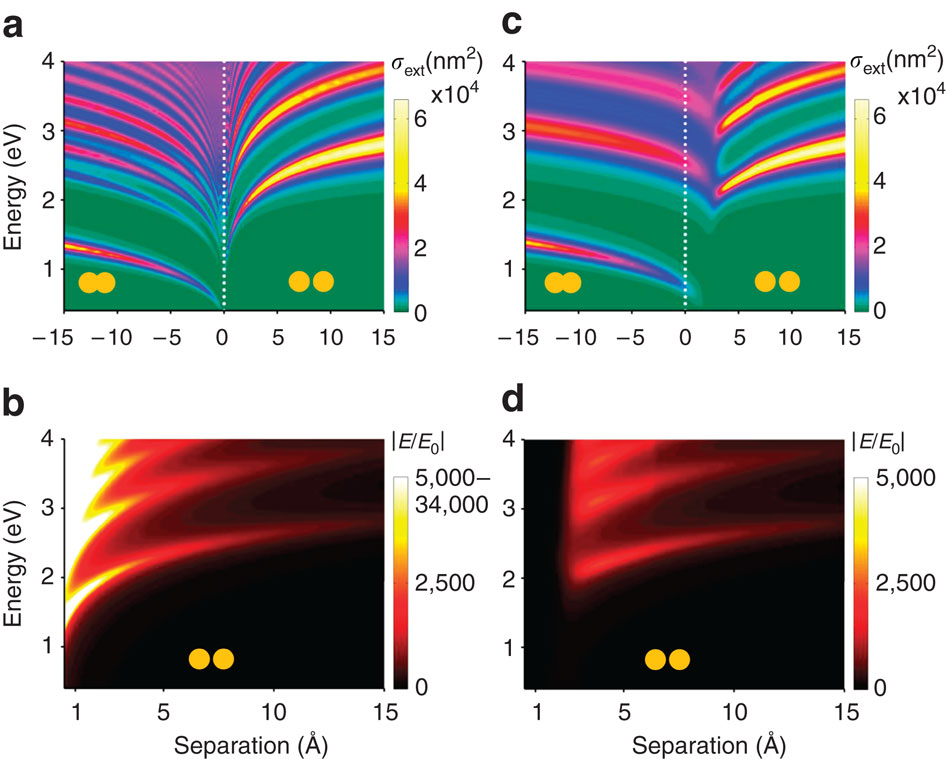
\includegraphics[width=0.7\textwidth, clip=true, trim=0 412 0 45]{figures/literature/ncomms1806-f4}\\
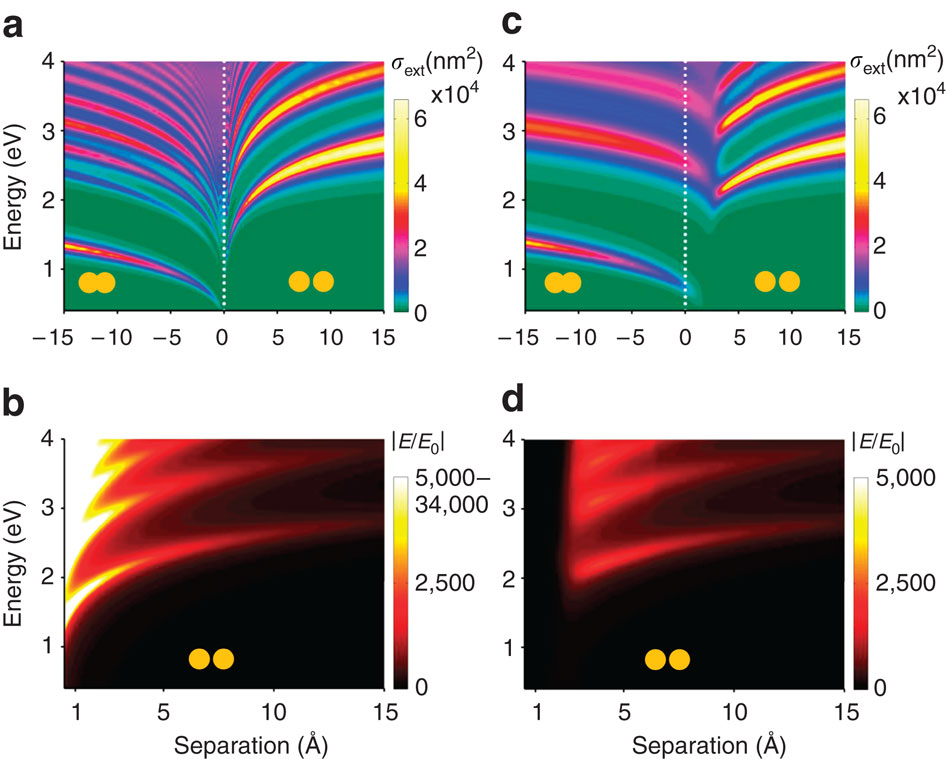
\includegraphics[width=0.7\textwidth, clip=true, trim=0 0 0 735]{figures/literature/ncomms1806-f4}
\caption[Numerical calculated extinction cross-section and field enhancement of a spherical AuNP dimer as a function of gap separation \cite{esteban2012}]{\textbf{Numerical calculated extinction cross-section and field enhancement of a spherical AuNP dimer as a function of gap separation \cite{esteban2012}.} The classical approach (left), valid for separations greater than $\sim$\SI{5}{\angstrom}, shows many modes redshifting into a singularity on geometrical contact, following by blueshifting CTP modes as the particles overlap. Introduction of an effective (conductive) gap medium to emulate the effects of quantum tunnelling (quantum corrected model, right) demonstrate the early onset of screening and CTP formation prior to geometrical contact. Figure taken from \cite{esteban2012}.}
\label{fig:optical_response_dimer}
\end{figure}

% Quantum Tunnelling
These classical predictions of plasmon coupling break down at small, sub-nm gaps where the continuum of excited higher order modes redshift to a singularity as $d\rightarrow0$, and the field enhancement increases infinitely. An example of classical calculations is shown in \figurename~\ref{fig:optical_response_dimer}, in which two AuNPs transition into contact. This behaviour is completely unphysical and is rectified once quantum mechanics is considered.
% Onset of tunnelling
Quantum mechanics begins to affect plasmon coupling under two conditions - either the particles become sufficiently small that quantum non-locality and non-local effects (finite, non-negligible electron wavefunction spill-out from the particle) become important or the gap size decreases to scales on which quantum tunnelling and non-locality of the gap surfaces can no longer be ignored. The onset of quantum tunnelling means charge is transported across the gap without requiring geometrical contact, rectifying the singularity predicted by classical electromagnetism.

The effects of quantum tunnelling were first predicted in small ($R<\SI{2}{nm}$) NaNPs using full quantum mechanical, time-dependent \gls{dft} calculations \cite{zuloaga2009}. Since these calculations consider the behaviour of each electron, they are currently limited in complexity to small systems containing less than 2000 electrons. Tunnelling effects in larger metallic nanostructures are predicted by the \gls{qcm}, a classical model which uses an effective gap dielectric function that takes into account the conductivity induced by quantum effects using pre-calculated values from \gls{dft} \cite{esteban2012}. Both the \gls{qcm} and TD\gls{dft} show agreement on the effects of tunnelling and conduction on plasmon coupling, with \gls{qcm} predictions for a AuNP dimer shown in \figurename~\ref{fig:optical_response_dimer}.

In numerical simulations, the onset of tunnelling creates a conductive bridge through which electrons pass during each half optical cycle. As particles approach the width and height of the potential barrier in the gap decreases as particle potentials begin to overlap, increasing the tunnelling probability. Charge transfer through the junction prevents the accumulation of charge on the surface and screens the electric field across the gap, thus reducing the coupling between plasmons and therefore the rate of redshift. This is the screening effect and is said to occur once in the ``crossover" regime, where the Fermi levels of each particle remain below the potential barrier \cite{zuloaga2009}. The reduction in the coupling strength means that higher order modes are not so easily excited and the continuum of modes seen in classical calculations no longer appears. The most prominent effect of screening is a drastic decrease of the field enhancement in the gap. In theory, this prevents small gaps from being useful as \gls{sers} structures, motivating the need to fully understand such effects. 

\begin{figure}[bt]
\centering
\fontsize{10pt}{1em}\selectfont
\def\svgwidth{0.65\textwidth}
\subimport{./figures/}{plasmon_contact.pdf_tex}
\caption[Diagram showing the emergence of charge transfer and screened bonding (crevice) plasmons on geometrical contact in a nanoparticle dimer]{\textbf{Diagram showing the emergence of charge transfer and screened bonding (crevice) plasmons on geometrical contact in a nanoparticle dimer.} The field generated by the bonding dimer plasmon (BDP) is screened from the gap by the conductive contact, forcing capacitive coupling to the crevice gap in the form of the screened bonding dimer plasmon (SBDP). The dominant charge oscillation is then the charge transfer plasmon (CTP) through the conductive bridge and across the whole structure.}
\label{fig:plasmon_contact}
\end{figure}

Upon increasing the tunnelling conductance by further decreasing the gap size, the dimers transition into a conductive regime. The Fermi level of each particle now sits above the potential barrier, allowing the free flow of electrons between particles and enabling \glspl{ctp} \cite{zuloaga2009}.%
\footnote{As per the Landau formalism for ballistic electron transport through a small constriction, the increase of the Fermi level above the barrier height enables a fixed number of conductance channels, each with a unit of quantum conductance, $\G0 = e^2/h$. This result is derived in the appendices.}
\Glspl{ctp} are plasmon resonances associated with charge oscillation through a conductive junction and multipolar resonances spread throughout the overall connected dimer structure. These are widely observed in geometrically contacted or overlapping plasmonic systems \cite{atay2004, lassiter2008}. Upon conductive contact, bonding modes in the gap are forced outwards to crevices, blueshifting in resonance position, diminishing in intensity and broadening in width as a result of significantly increased screening currents. A dipolar \gls{ctp} emerges at lower energies as screened $l=i$ hybridised plasmons transition into $l=i+1$ \glspl{ctp} due to their similar charge distributions \cite{romero2006, perez2010, tserkezis2014}. The lower energies of \glspl{ctp} are associated with a spatially larger dipole, as shown in \figurename~\ref{fig:plasmon_contact}, which indicates that they blueshift with increasing particle overlap.%
\footnote{For a spherical \gls{mnp} dimer with a \gls{bdp} and \gls{bqp} the corresponding \gls{ctp} modes are typically labelled as the \gls{ctp} and CTP$^\prime$. The CTP$^\prime$ is often labelled as the \gls{sbdp} due to the similarities in the charge distributions between a second order CTP and first order bonding mode.}

\begin{figure}[bt]
\centering
\vspace{-10pt}
\begin{tikzpicture}
\node [below left] at (0,0) {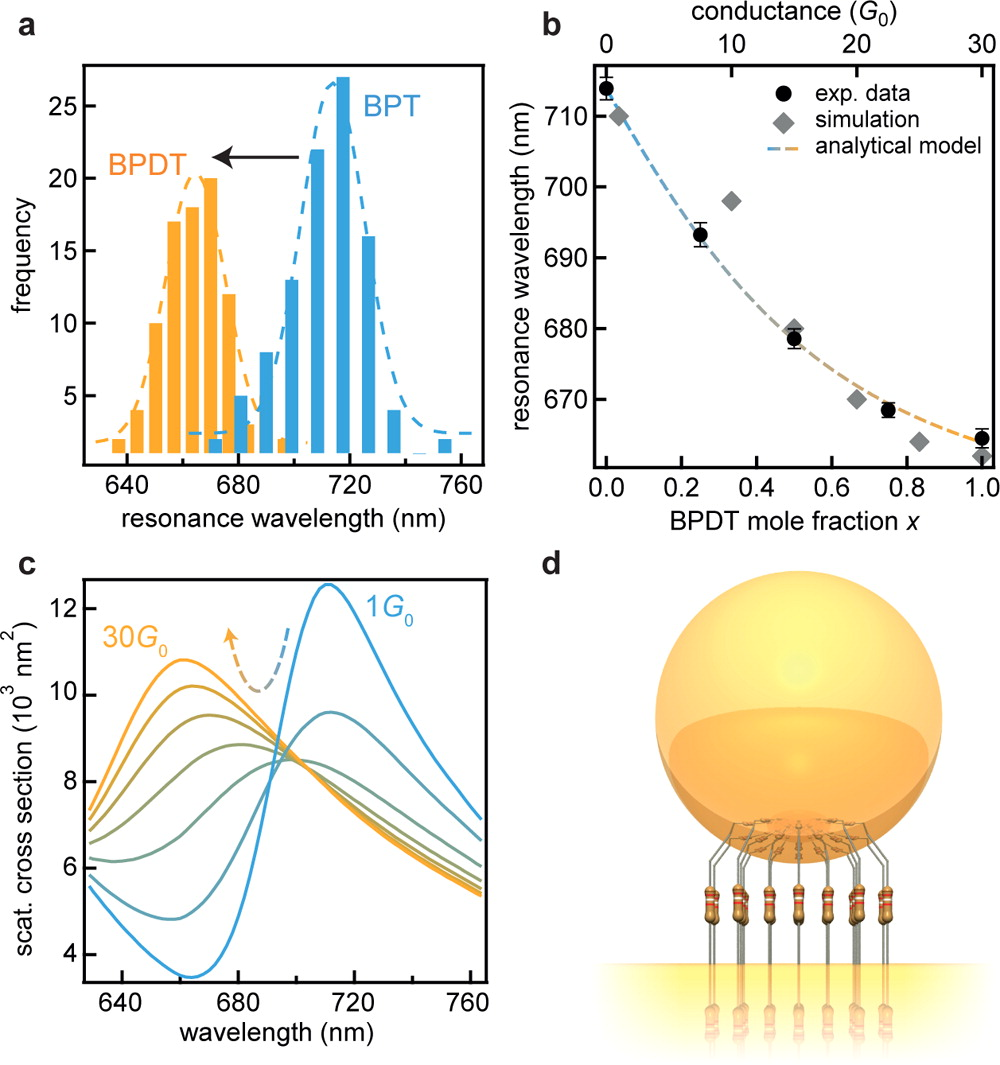
\includegraphics[width=6cm, clip=true, trim=0 125 123 15]{figures/literature/nl-2014-041786_0003}};
\node [below right] at (0,0) {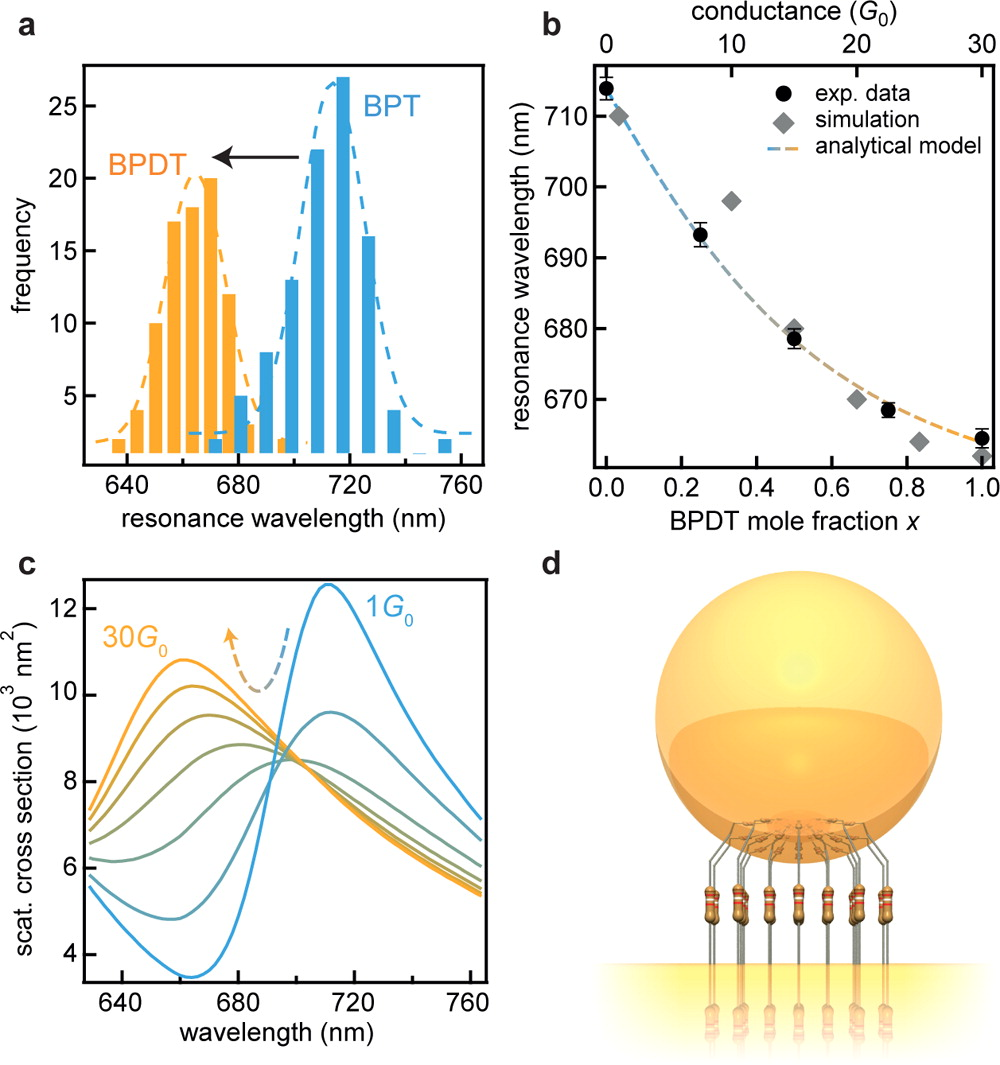
\includegraphics[width=6cm, clip=true, trim=0 4 123 138.5]{figures/literature/nl-2014-041786_0003}};
\node [below left] at (-5.5,0.1) {(a)};
\node [below left] at (0.8,0.1) {(b)};
\end{tikzpicture}
\caption[Experimental and theoretical scattering spectra of \SI{80}{nm} AuNP dimers connected via variable conductance molecular linkers \cite{benz2014}]{\textbf{Experimental and theoretical scattering spectra of \SI{80}{nm} AuNP on a planar Au mirror separated via variable conductance molecular spacer layer \cite{benz2014}.} Variable conductance molecular SAMs are formed from fractional mixing of BPT (insulating) and BPDT (conductance). The blueshift and attenutation of the coupled plasmon begins at 2\G0 with the screened mode emerging once $G>5\G0$.}
\label{fig:benz_molecular_npom}
\vspace{-5pt}
\end{figure}

Both the blueshifting portion of the screening effect and \gls{ctp} excitation require a conductance threshold to be surpassed in order for these effects to occur. Thresholds have been defined for a dimer containing a classical conductive linker, where the gap between particles of radius $R$ has a width $d$, conductivity $\sigma$ and linker radius $a$ \cite{perez2010}. The formation of screened plasmons occurs at low conductances whereas a higher junction conductance is required for CTP excitation. The conductance threshold for screening of the dipolar bonding plasmon is given by,
\begin{subequations}
\begin{equation}
	G_{\mathrm{SBDP}} = 2\epsfs\omega_{\mathrm{BDP}}\frac{a^2}{d}.
\end{equation}
The conductance can be reduced to a conductivity threshold by removing a factor of $\pi a^2/d$ yielding,
\begin{equation}
	\sigma_{\mathrm{SBDP}} = 2\epsfs\frac{\omega_{\mathrm{BDP}}}{\pi}.
\end{equation}
\end{subequations}
The threshold is intrinsically independent of geometry and depends only on the conductivity. For larger contact widths or shorter linker lengths the threshold increases to overcome the increased capacitive coupling. Experiments maintaining a fixed geometry whilst increasing the gap conductivity using fractional mixing of similar conductive and insulating \glspl{sam} have succeeded in showing a blueshift of coupled plasmons with an estimated 2\G0 threshold \cite{benz2014}, as shown in \figurename~\ref{fig:benz_molecular_npom}. A similar 2\G0 threshold is also found in theoretically considered \SI{1}{nm} dimer linkers \cite{perez2010}.

% CTP effect
A second, much larger, threshold exists for \gls{ctp} formation, occurring at,
\begin{subequations}
\begin{equation}
	G_{\mathrm{CTP}} = \epsfs\omega_{\mathrm{CTP}}\frac{R^2}{d},
\end{equation}
which can similarly be reduced to a conductivity threshold,
\begin{equation}
	\sigma_{\mathrm{CTP}} = \epsfs \frac{\omega_{\mathrm{CTP}}}{\pi} \left(\frac{R}{a}\right)^2.
\end{equation}
\end{subequations}
Unlike screening, \gls{ctp} formation depends not only on the conductivity but the junction geometry. The geometry factor $(R/a)$ represents the ratio between the total charge in the particle and the amount which can pass through a gap with fixed conductivity. Having a large conductivity means the junction does not have to be as wide, relative to the particle size, to accommodate enough current to maintain a \gls{ctp}. Hence, dimers linked by a highly conductive metallic link can sustain a \gls{ctp} with only a small nanometric-scale contact area. This has been demonstrated by threading together AuNP dimers fixed with a hollow spacer molecule using high power laser pulses \cite{herrmann2014, tserkezis2014}. % resulting in Au linkers of various widths

%For a fixed linked dimer geometry the optics can be controlled through the gap conductivity. Increasing the conductivity leads to screening, and therefore blueshifting, of the bonding mode before a \gls{ctp} emerges \cite{perez2011, zabala2011}. Since the geometry does not change the \gls{ctp}, once excited, does not tune and the blueshift of the screened mode saturates.
%Under these conditions, screening occurs as expected and the \gls{ctp} energy increases with linker width \cite{perez2011}. Dimers in which the gap width changes, leading to overlap, form a more complex system to understand since the geometrical changes also influence the plasmonics along with charge transfer.

%Once particles come into geometrical contact and begin to form a metallic (ballistic or ohmic) contact

\begin{figure}[bt]
\centering
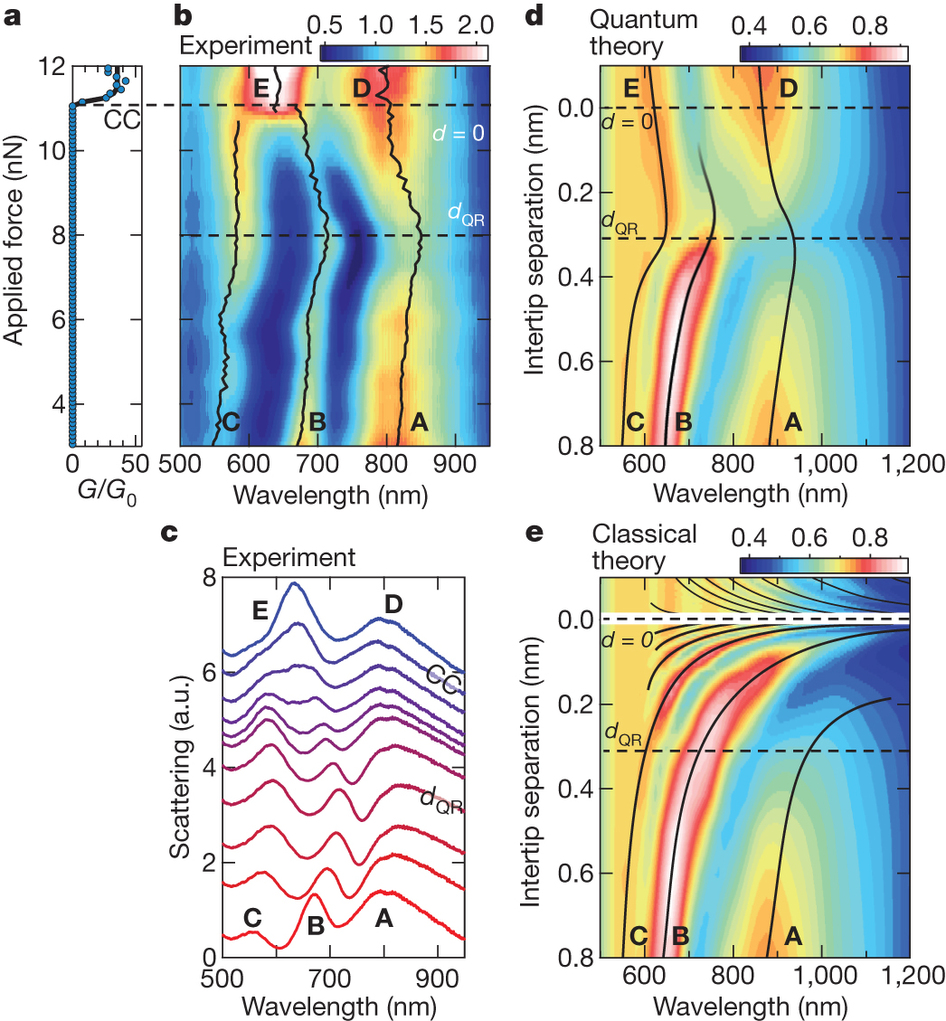
\includegraphics[width=0.65\textwidth, clip=true, trim=0 500 0 0]{figures/literature/nature11653-f2_2}\\
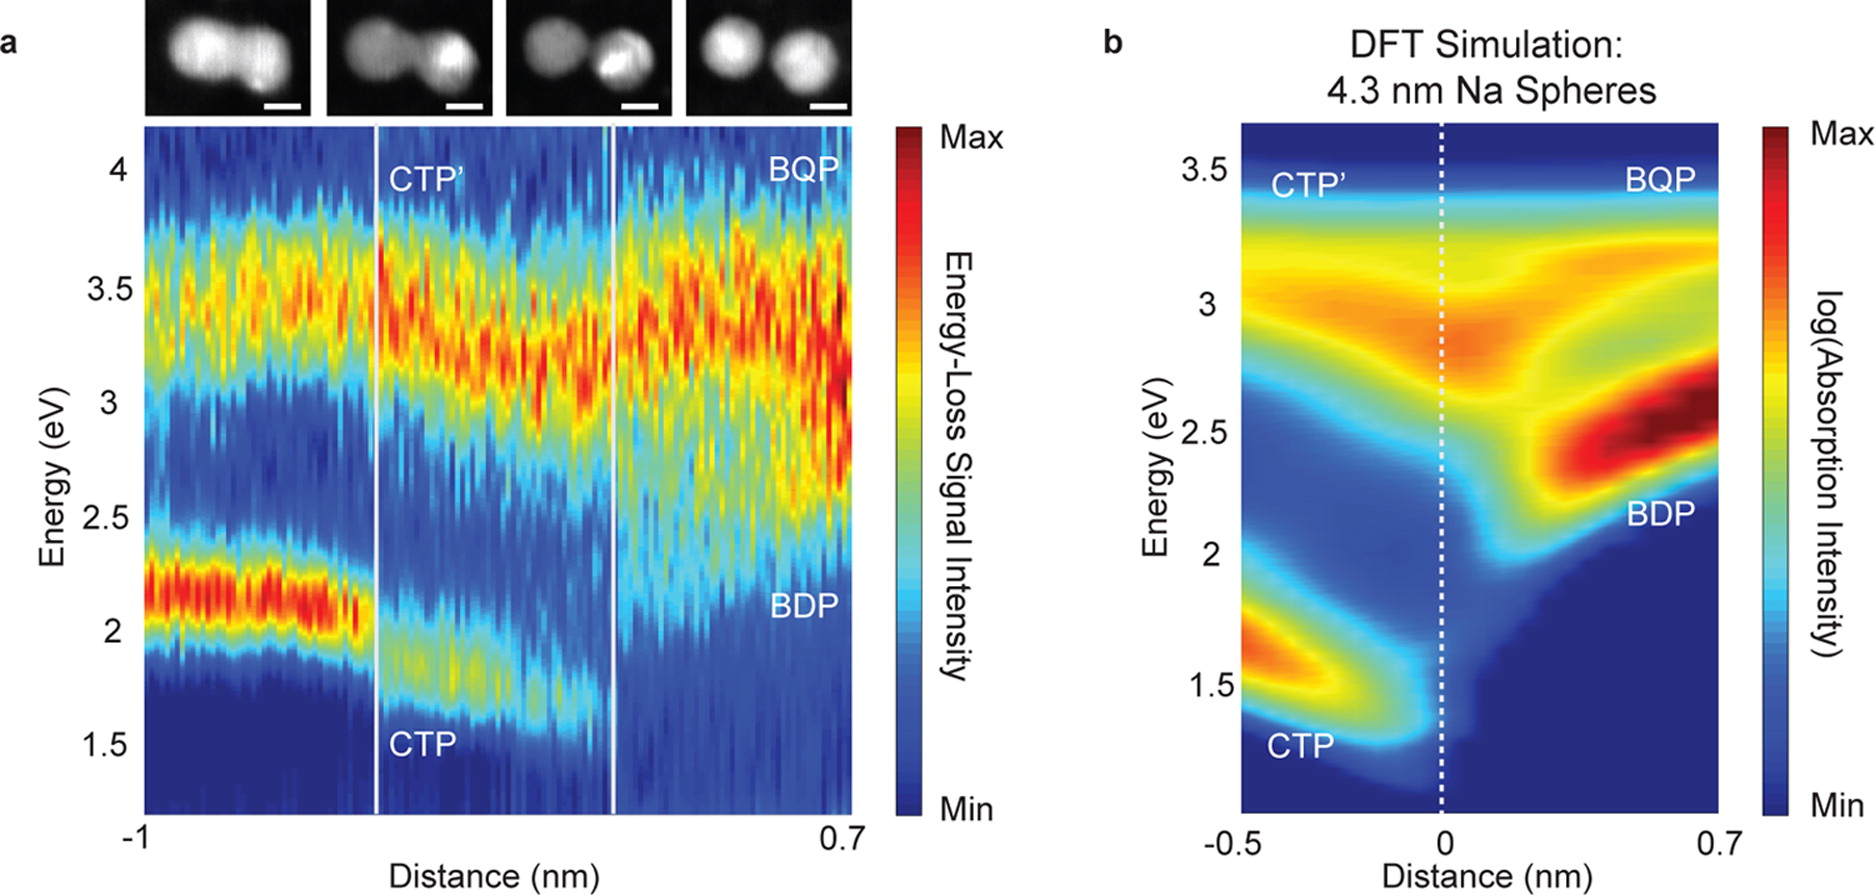
\includegraphics[width=0.65\textwidth]{figures/literature/nl-2012-04078v_0001}
\caption[Examples of experimental measurements of the effect of quantum tunnelling on plasmonic gap systems]{\textbf{Examples of experimental measurements of the effect of quantum tunnelling on plasmonic gap systems through direct monitoring of the plasmon resonances.} (top) Supercontinuum dark-field scattering measurements of two \SI{300}{nm} diameter spherical Au tips in a dimer configuration with reducing separation, transitioning below \SI{1}{nm} and into the quantum regime \cite{savage2012}. (bottom) EELS measurements of \SI{10}{nm} AgNPs being induced closer together by the electron beam \cite{scholl2013}.}
\label{fig:tunnelling_plasmonics}
\end{figure}

% Experimental measurements
Experimental evidence for each of the predicted effects of quantum tunnelling in plasmonic systems has recently been found using optical spectroscopy \cite{savage2012, cha2014, zhu2014}, \gls{eels} \cite{scholl2013}, \gls{sers} \cite{zhu2014}, photoluminescence \cite{kravtsov2014} and third-harmonic generation measurements \cite{hajisalem2014}.
% Direct measurements
Preliminary measurements were made using optical scattering from a dynamic spherically-tipped Au AFM probe dimer, with simulated spectra using the \gls{qcm} (\figurename~\ref{fig:tunnelling_plasmonics}) \cite{savage2012}. Plasmon modes are shown to blueshift upon decreasing past a critical separation of \SI{0.3}{nm}. Scattering spectra qualitatively agreed with the \gls{qcm}, with discrepancies attributed to difficulty in simulating an extended dual tip geometry. Better agreement with \gls{dft} calculations was found in \gls{eels} measurements on \SI{10}{nm} AgNP dimers, brought together under the influence of the electron beam (\figurename~\ref{fig:tunnelling_plasmonics}) \cite{scholl2013}. In this instance the characteristic screening blueshift occurred at $\sim$\SI{0.5}{nm}. Both experiments confirm that \glspl{ctp} only appear after geometrical contact, when the conductance can rise sufficiently.

% Molecular distance tuning - note this is not the best quality data or papers
Alkanedithiol molecules of various lengths have also been used to discretely tune the gap separation of AuNP dimers \cite{cha2014}. In this case, blueshifting and attenuation of the bonding dipolar plasmon, as well as an increase in its width, is measured with molecules smaller than pentanedithiol. Similar results are found when using intercalating \glspl{sam} \cite{tan2014}.
% Inferred measurements
Further investigations into sub-nm plasmonic gaps have also shown behaviours attributed to quantum tunnelling, though inferred from properties depending on the field enhancement as opposed to direct measurement of \glspl{spr}. A decrease in signal intensity in both the \gls{sers} peaks \cite{zhu2014} and photoluminescence \cite{kravtsov2014} in nano-gap systems, for example, are signatures of quantum tunnelling screening the coupled plasmon field.

\begin{figure}[bt]
\centering
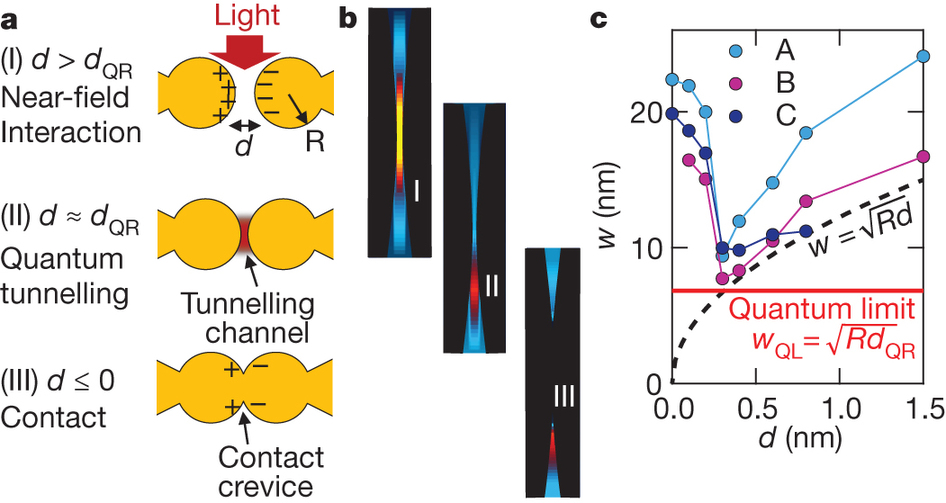
\includegraphics[width=0.6\textwidth]{figures/literature/nature11653-f3_2}
\caption[Plasmon mode distributions in the quantum regime]{\textbf{Plasmon mode distributions in the quantum regime.} Diagram showing the different regimes of plasmonic interaction, taken from \cite{savage2012}. The onset of a tunnelling current pinches of the electric field in the gap via screening/conductive losses prior to conductive contact, which shows a similar expulsion of field from the gap.}
\label{fig:savage2012c}
\end{figure}

Interestingly, qualitative agreement between \gls{qcm} calculations and full quantum mechanical calculations suggest that the quantum nature of the system is of little importance. Even though the \gls{qcm} uses a classical, resistive gap with conductances values characteristic of quantum tunnelling followed by ballistic conduction, the effects on gap plasmons caused by quantum charge transport are accurately replicated. This implies that, despite the quantum nature of such small gaps, the effects of quantum charge transport on plasmon coupling depend only on the amount of charge transfer and not the mechanism by which it occurs. This links together work done using particle positioning \cite{savage2012, scholl2013} with studies of interacting plasmonic system coupled with molecular linkers \cite{tan2014, cha2014, benz2014}. Quantum tunnelling and non-geometrical conductance still remains an interesting case, however, since both forms of conduction are unavoidable once gap sizes decrease below \SI{0.5}{nm}. This is why the point at which the electric field is expelled from the gap is described as the quantum limit to plasmon confinement \cite{savage2012}. For this reason, it is important to fully understand the relations between plasmonic hot spots and sites of (quantum) charge transfer.

\end{document}